\section{Metod}
Först undersöktes de strukturella förbättringarna som har föreslagits i biblioteket och sedan de algoritmiska.
\subsection{Strukturella förbättringar}
Tidigare så föreslogs att matrisernas L och U matriser kunde sparas i matrix-structen så dessa inte behövdes beräknas varje gång. Detta fungerar bra så länge matrisen inte ändras och då detta behövs då kollas i alla funktioner som ändrar på matrisens innehåll. Så structen skulle isåfall innehålla två extra matriser och en booleank variabel som höll koll på om matrisen ändrades. Att testa i alla funktioner bestämdes till att vara väldigt överflödigt och om någon lägger till en funktion och glömmer lägga in testet så faller hela konceptet. Samma sak gäller om någon väljer att manipulera datan i matrisen direkt utan att använda bibliotekets funktioner så detta alternativ gick bort.

\subsection{Algoritmiska förbättringar}
Den förbättringen som valdes till den bästa för biblioteket var att använda strassen istället för den naiva algoritmen när man utförde matrismultiplikationer. Först så implementerades algoritmen och sedan så gjordes tester för att bestämma när det blev mer optimerat att använda den istället för den naiva. I den nuvarande implementation så används funktionen multiply\_matrices som innehåller den naiva algoritmen. Detta gjordes om så att den funktionen kallar på multiply\_matrices\_naive om storleken på den resulterande matrisen understiger gränsvärdet som mättes upp , annars kallar funktionen på strassen\_matrices för matrismultiplikation. 
\\
\\
För att sedan testa om biblioteket kunde utnyttja en paralleliserad version av Strassen så implementerades  strassen\_matrices\_parallel. Dock för att bibehålla kompabiliteten med alla platformen så kan all denna kod tas bort av preprocessorn genom att inte sätta PARALLEL flaggen i matLib.h
\subsection{Implementation av Strassen algoritmen}
Implementationen använder algoritmen beskriven i \ref{sec:strassen}. Dock beroende på utformning av bibliotektet så måste en ny matris skapas för varje operation man gör. Detta leder till att under en multiplikation utan rekursivt anrop så skapas och frigörs 38 matriser. 

\subsection{Jämförelser mellan algoritmer}
I figur~\ref{fig:comparison} kan man se jämförelsen mellan Strassen och naive. Upplösningen mellan punkter är rätt dålig men det tar lång tid att beräkna punkter över 500 element. Datan är dock genomsnittet av 5 tester per algoritm. Man kan tydligt se att över 500 element så har Strassen ett stort övertag över naive. 

\begin{figure}[H]
	\begin{center}
		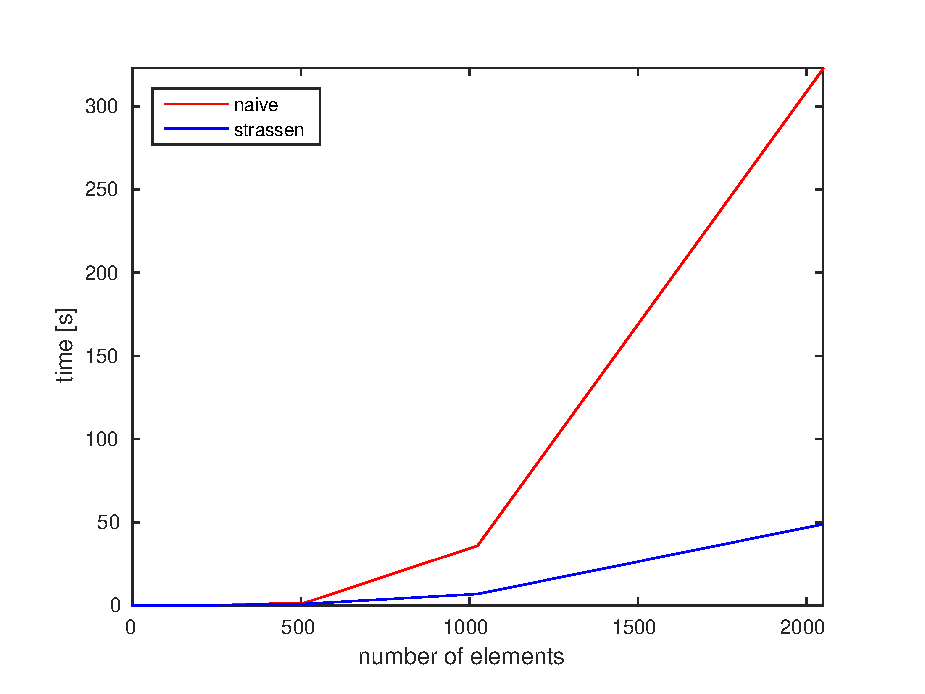
\includegraphics[scale=0.6]{martin-tex/comparison.eps}
	\end{center}
	\caption{Jämförelse mellan naive och Strassen.}
	\label{fig:comparison}
\end{figure}

\subsection{Implementation av Strassen paralelliserad}
Implementation använder algoritmen beskriven i \ref{sec:strassen}. Det som sker nu är att varje gång någon av matriserna $M_{1-7}$ ska beräknas och om det finns en ledig tråd så körs detta i den. Annars beräknas den i den nuvarande tråden. För att hålla koll på antalet trådar som körs så finns den globala räknaren thread\_counter som skyddas av ett lås för att försäkra ömsesidig uteslutning. Maximala antalet trådar sätts i den statiska variabeln number\_of\_cores. När någon nuvarande tråd kommer till ett tillfälle den den ska beräkna någon av 
$M_{1-7}$ så låser den thread\_counter och jämför denna med number\_of\_cores och om dessa är olika så beräknas multiplikationen med strassen\_matrices\_parallel. Detta skapar en ny tråd för beräkningen. Annars så utförs beräkning med strassen\_matrices som då sker i den nuvarande tråden.

\subsection{Jämförelse mellan paralleliserad och oparalleliserad Strassen}
Jämförelsen är svår att göra då man kan variera båda antalet element och antalet trådar som processen använder. När tidigare tidsmätningar har gjorts så har c-bibliotket time.h användts men detta mäter den effektiva cpu-tiden. När man använder fler trådar så är detta missvisande då det intressanta är reela tiden det tar. För att lösa detta så används bash kommandot time för att mäta tiden istället. Resultatet från jämförelsen kan ses i figur~\ref{fig:threads}. Detta test utfördes på en bärbar dator med en tvåkärning I7 processor med Hyper threading vilket gör att det kan jämföras med en fyrakärnig processor. Helst skulle testet utförts på en dator med fler kärnor. I figur~\ref{fig:threads} kan man se en tydlig prestande ökning från vanliga algoritmen till algoritmen när den använder en extra tråd. Därefter avtar prestandeökning. Att multiplicera 2 matriser som var 4096x4096 tog 582 sekunder med den vanliga och som bäst 343 sekunder när den använda 16 trådar. Samma beräkning med den naiva algoritmen tog 2688.527 sekunder. 

\begin{figure}[H]
	\begin{center}
		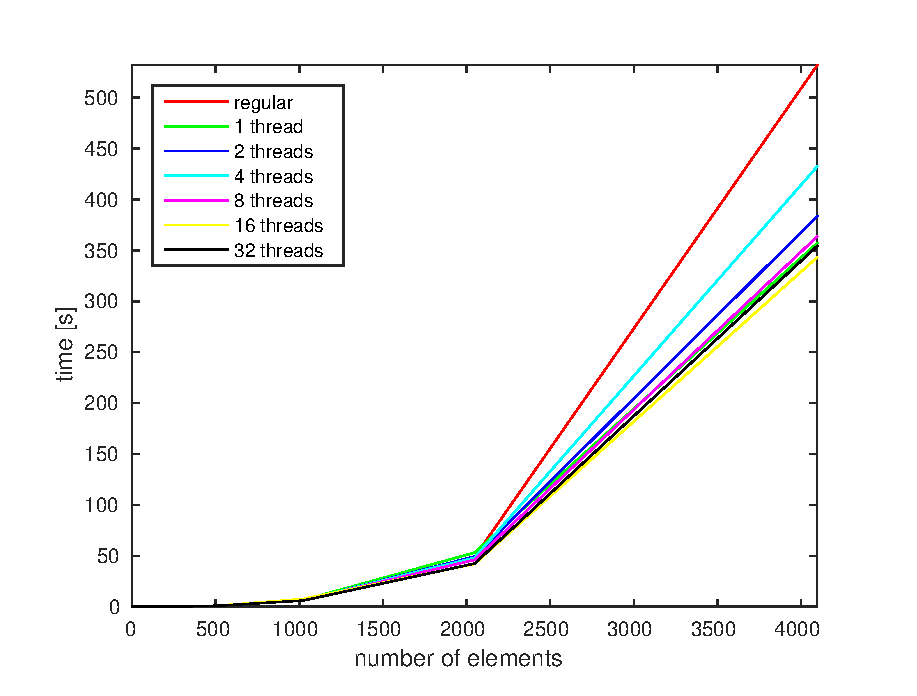
\includegraphics[scale=0.6]{martin-tex/threads_test.eps}
	\end{center}
	\caption{Jämförelse mellan vanliga Strassen och parallel version.}
	\label{fig:threads}
\end{figure}


